\documentclass[reprint,english,notitlepage]{revtex4-2}

\usepackage[utf8]{inputenc}
\usepackage[english]{babel}

\usepackage{physics,amssymb}
\usepackage{graphicx}
\usepackage{xcolor}
\usepackage{hyperref}
\usepackage{tikz}
\usepackage{listings}
\usepackage{subfigure}
\graphicspath{ {/Users/rebeccanguyen/Documents/GitHub/H22} }

\hypersetup{
    colorlinks,
    linkcolor={red!50!black},
    citecolor={blue!50!black},
    urlcolor={blue!80!black}}


\lstset{
	inputpath=,
	backgroundcolor=\color{white!88!black},
	basicstyle={\ttfamily\scriptsize},
	commentstyle=\color{magenta},
	language=Python,
	morekeywords={True,False},
	tabsize=4,
	stringstyle=\color{green!55!black},
	frame=single,
	keywordstyle=\color{blue},
	showstringspaces=false,
	columns=fullflexible,
	keepspaces=true}

\begin{document}
\title{Temperfect mug}   % self-explanatory
\author{Rebecca Nguyen}               % self-explanatory
\date{\today}                             % self-explanatory
\noaffiliation
\maketitle                                % creates the title, author, date & abstract


% the fundamental components of scientific reports:
\section{Introduction}
The Temperfect mug has an extra layer of insulation which brings your hot beverage
to a more pleasant temperature, allowing you to enjoy your freshly-brewed drink right away.
We want to better understand this mug by conducting an experiment where the
cooling of beverage will be measured. The experiment will be conducted on both the Temperfect mug and Bodum thermos cup.

\section{Theory}
The multiplicity in an Einstein solid is given by
\begin{equation}
  \Omega(N, q) \approx \frac{(q+N)!}{q!N!}
\end{equation}
Entropy
\begin{equation}
  S \equiv k \ln\Omega
\end{equation}
Total energy of the solid
\begin{equation}
  U = \frac{N}{2}\epsilon + q\epsilon
\end{equation}
Which results in
\begin{equation}
  \frac{dU}{dq} = \epsilon \rightarrow dU = \epsilon dq
\end{equation}
dU = Tds - pdv \\
C_v = \frac{dU}{dT}

\section{Method}
The Temperfect mug and Bodum thermos cup were both filled with 3dl of almost boiling water. The lids were not put on to allow temperature logging while the water in the mugs cooled. The temperature in the air outside of the mug was $T_a = 22^{\circ}$.

\section{Results}

\begin{figure}
  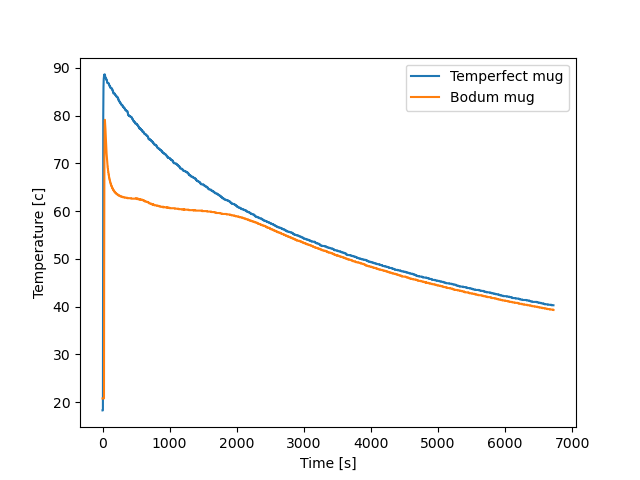
\includegraphics[scale=0.5]{temperature.png}
  \caption{Temperature against time of both mugs}\label{figure}
\end{figure}

\section{Discussion}
\section{Conclusion}

\begin{acknowledgments}
I would like thank myself for writing this beautiful document.
\end{acknowledgments}


%% When it comes to the bibliography I personally generate it using BibLaTeX. (see the link above if you're interested)
%% You're obviously allowed to create the references section however you like.
%% I'll keep it simple here.
\section*{References}  % the asterisk (*) after \section makes the section numbering go away
\begin{itemize}
\item[-]Reference 1
\item[-]Reference 2
\end{itemize}

\newpage
%% if you want to include an appendix, this is how you do it
\appendix
\section{Name of appendix}
This will be the body of the appendix.
\section{This is another appendix}\label{appendix}
Tada.
%% all \section commands following \appendix are automatically taken as appendices

%% Note that \label{appendix} command on line 115. What this does is setup a reference point for LaTeX that you can
%% access wherever you want using \ref{appendix}.
%% You can place labels on most environments such as equations, figures, tables, etc.

\clearpage
Note that this document is written in the two-column format. If you want to display a large equation, a large figure, or whatever, in one-column format, you can do this like so:
\onecolumngrid
\vspace{1cm} % some extra space
This text and this equation are both in one-column format.

\footnote{This equation is actually from quantum mechanics. ``It's called Schrödinger's Time-Dependent Wave Equation'', named after the awesome Austrian physicist Erwin Rudolf Josef Alexander Schrödinger. Yep, the ``Schrödinger's cat'' guy. Pretty cool dude actually, check his wiki page: \url{https://en.wikipedia.org/wiki/Erwin_Schrodinger}. He was physics' no. 1 Ladies' man if there ever was one. Anyway, you will learn more about this equation in FYS2140. You can also find it printed on a glass wall in the UiO Physics Building (it really is that important).}

\begin{equation}\label{equation}
\frac{-\hbar^2}{2m}\laplacian{\Psi}+V\Psi=i\hbar\pdv{t}\Psi
\end{equation}
Note that the equation numbering (this: \ref{equation}) follows the appendix as this text is technically inside Appendix \ref{appendix}. If you want a detailed listing of (almost) every available math command, check: \url{https://en.wikibooks.org/wiki/LaTeX/Mathematics}.
\vspace{1cm} % some extra space
\twocolumngrid
And now we're back to two-column format. It's really easy to switch between the two. It's recommended to keep the two-column format, because it is easier to read, it's not very cluttered, etc. Pro Tip: You should also get used to working with REVTeX because it is really helpful in FYS2150.

One last thing, this is a code listing:
\begin{lstlisting}
This will be displayed with a cool programming font!
\end{lstlisting}
You can add extra arguments using optional parameters:
\begin{lstlisting}[morekeywords={cool}]
This will be displayed with a cool programming font!
\end{lstlisting}
You can also list code from a file using \texttt{lstinputlisting}. If you're interested, check \url{https://en.wikibooks.org/wiki/LaTeX/Source_Code_Listings}.

This is a basic table:
\begin{table}[h]  % h = "here"  , h! = here!
\caption{This is a nice table}\label{table}
\begin{tabular}{|c|c|c|} % note that & separates columns while \\ separates the rows
\hline                    % creates a horizontal line (try removing it)
Hey & Hey & Hey  \\
\hline
Hello & Hello & Hello \\
\hline
Bye & Bye & Bye \\
\hline
\end{tabular}
\end{table}\\
You can a detailed description of tables here: \url{https://en.wikibooks.org/wiki/LaTeX/Tables}.

This is a more advanced table:
%tabell i latex
\begin{table}[h!] %%h! er for å tvinge tabellen til å være nærmest mulig her i dokumentet
  \begin{center}
    \caption{Tabelleksempel} %Tabelltekst
    \label{tab:results}
    \begin{tabular}{l|c|r} % for hver kolonne har du {a|b|c} der a er for 1.kolonne, b for 2. kolonne etc, l=venstrestil, r=høyrestilt, c = senterstilt. Se posisjonen til tallene i de forskjellige kolonnene. Har du 4 kolonner der alle er senterstilt blir det f.eks. {c|c|c|c}
      \textbf{Partikkelindeks} & \textbf{Posisjon} & \textbf{Hastighet}\\ %innhold i hver kolonne, legg til flere her hvis du har flere kolonner
      (i) & (m) & (m/s)\\ %enheter for hver kolonne
      \hline %en horisontall linje for å skille overskriften fra tallene under. Vil du ha en slik linje mellom hver rad i tabellen så legg til en \hline mellom hver rad nedover her. Merk \\ er som vanlig linjeskift mens & skiller kolonner
      0 & 139.22 & 12.4\\
      1 & 14.88 & 18.7\\
      2 & 233.9 & 10.10\\
      3 & 816.12 & 13.4\\
      \hline
    \end{tabular}
  \end{center}
\end{table}



I'm not going to delve into Tikz in any level detail, but here's a quick picture:
\begin{figure}[h]
\centering  % places the tikz image in the center of the text column
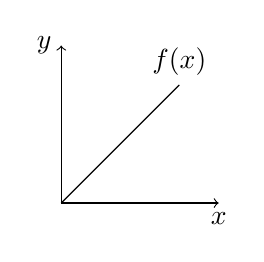
\begin{tikzpicture}
\draw[->] (0,0) -- (2,0) node [pos=1.0,below] {\(x\)};
\draw[->] (0,0) -- (0,2) node [pos=1.0,left] {\(y\)};
\draw (0,0) -- (1.5,1.5) node [pos=1.0,above] {\(f(x)\)};
\end{tikzpicture}
\caption{This is great caption}\label{figure}
\end{figure}\\
If you want to know more, check: \url{https://en.wikibooks.org/wiki/LaTeX/PGF/TikZ}.

%% If you want to include figure:
%\includegraphics[scale=1.0]{filename}
%% check https://en.wikibooks.org/wiki/LaTeX/Importing_Graphics if you want to know more

\end{document}
